\documentclass[1p]{elsarticle_modified}
%\bibliographystyle{elsarticle-num}

%\usepackage[colorlinks]{hyperref}
%\usepackage{abbrmath_seonhwa} %\Abb, \Ascr, \Acal ,\Abf, \Afrak
\usepackage{amsfonts}
\usepackage{amssymb}
\usepackage{amsmath}
\usepackage{amsthm}
\usepackage{scalefnt}
\usepackage{amsbsy}
\usepackage{kotex}
\usepackage{caption}
\usepackage{subfig}
\usepackage{color}
\usepackage{graphicx}
\usepackage{xcolor} %% white, black, red, green, blue, cyan, magenta, yellow
\usepackage{float}
\usepackage{setspace}
\usepackage{hyperref}

\usepackage{tikz}
\usetikzlibrary{arrows}

\usepackage{multirow}
\usepackage{array} % fixed length table
\usepackage{hhline}

%%%%%%%%%%%%%%%%%%%%%
\makeatletter
\renewcommand*\env@matrix[1][\arraystretch]{%
	\edef\arraystretch{#1}%
	\hskip -\arraycolsep
	\let\@ifnextchar\new@ifnextchar
	\array{*\c@MaxMatrixCols c}}
\makeatother %https://tex.stackexchange.com/questions/14071/how-can-i-increase-the-line-spacing-in-a-matrix
%%%%%%%%%%%%%%%

\usepackage[normalem]{ulem}

\newcommand{\msout}[1]{\ifmmode\text{\sout{\ensuremath{#1}}}\else\sout{#1}\fi}
%SOURCE: \msout is \stkout macro in https://tex.stackexchange.com/questions/20609/strikeout-in-math-mode

\newcommand{\cancel}[1]{
	\ifmmode
	{\color{red}\msout{#1}}
	\else
	{\color{red}\sout{#1}}
	\fi
}

\newcommand{\add}[1]{
	{\color{blue}\uwave{#1}}
}

\newcommand{\replace}[2]{
	\ifmmode
	{\color{red}\msout{#1}}{\color{blue}\uwave{#2}}
	\else
	{\color{red}\sout{#1}}{\color{blue}\uwave{#2}}
	\fi
}

\newcommand{\Sol}{\mathcal{S}} %segment
\newcommand{\D}{D} %diagram
\newcommand{\A}{\mathcal{A}} %arc


%%%%%%%%%%%%%%%%%%%%%%%%%%%%%5 test

\def\sl{\operatorname{\textup{SL}}(2,\Cbb)}
\def\psl{\operatorname{\textup{PSL}}(2,\Cbb)}
\def\quan{\mkern 1mu \triangleright \mkern 1mu}

\theoremstyle{definition}
\newtheorem{thm}{Theorem}[section]
\newtheorem{prop}[thm]{Proposition}
\newtheorem{lem}[thm]{Lemma}
\newtheorem{ques}[thm]{Question}
\newtheorem{cor}[thm]{Corollary}
\newtheorem{defn}[thm]{Definition}
\newtheorem{exam}[thm]{Example}
\newtheorem{rmk}[thm]{Remark}
\newtheorem{alg}[thm]{Algorithm}

\newcommand{\I}{\sqrt{-1}}
\begin{document}

%\begin{frontmatter}
%
%\title{Boundary parabolic representations of knots up to 8 crossings}
%
%%% Group authors per affiliation:
%\author{Yunhi Cho} 
%\address{Department of Mathematics, University of Seoul, Seoul, Korea}
%\ead{yhcho@uos.ac.kr}
%
%
%\author{Seonhwa Kim} %\fnref{s_kim}}
%\address{Center for Geometry and Physics, Institute for Basic Science, Pohang, 37673, Korea}
%\ead{ryeona17@ibs.re.kr}
%
%\author{Hyuk Kim}
%\address{Department of Mathematical Sciences, Seoul National University, Seoul 08826, Korea}
%\ead{hyukkim@snu.ac.kr}
%
%\author{Seokbeom Yoon}
%\address{Department of Mathematical Sciences, Seoul National University, Seoul, 08826,  Korea}
%\ead{sbyoon15@snu.ac.kr}
%
%\begin{abstract}
%We find all boundary parabolic representation of knots up to 8 crossings.
%
%\end{abstract}
%\begin{keyword}
%    \MSC[2010] 57M25 
%\end{keyword}
%
%\end{frontmatter}

%\linenumbers
%\tableofcontents
%
\newcommand\colored[1]{\textcolor{white}{\rule[-0.35ex]{0.8em}{1.4ex}}\kern-0.8em\color{red} #1}%
%\newcommand\colored[1]{\textcolor{white}{ #1}\kern-2.17ex	\textcolor{white}{ #1}\kern-1.81ex	\textcolor{white}{ #1}\kern-2.15ex\color{red}#1	}

{\Large $\underline{12n_{0624}~(K12n_{0624})}$}

\setlength{\tabcolsep}{10pt}
\renewcommand{\arraystretch}{1.6}
\vspace{1cm}\begin{tabular}{m{100pt}>{\centering\arraybackslash}m{274pt}}
\multirow{5}{120pt}{
	\centering
	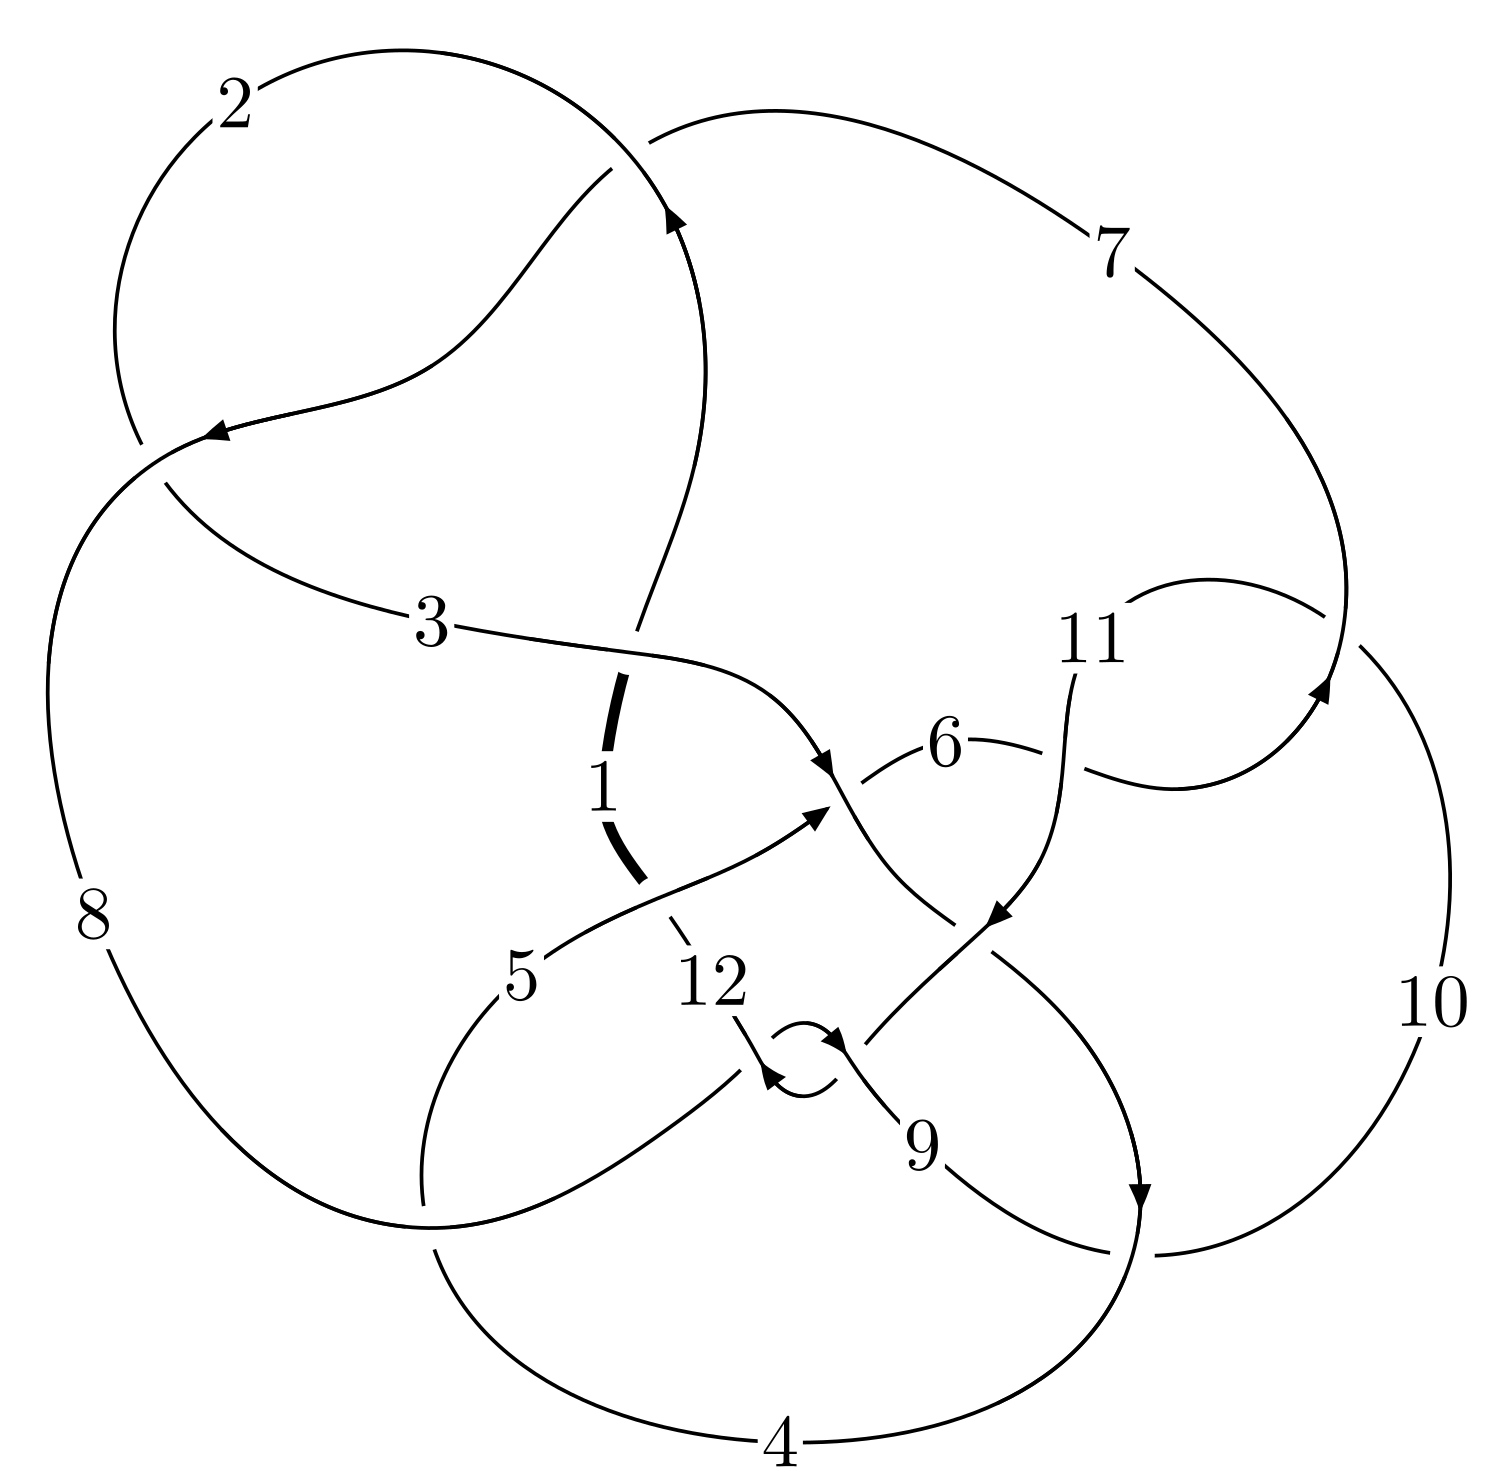
\includegraphics[width=112pt]{../../../GIT/diagram.site/Diagrams/png/2713_12n_0624.png}\\
\ \ \ A knot diagram\footnotemark}&
\allowdisplaybreaks
\textbf{Linearized knot diagam} \\
\cline{2-2}
 &
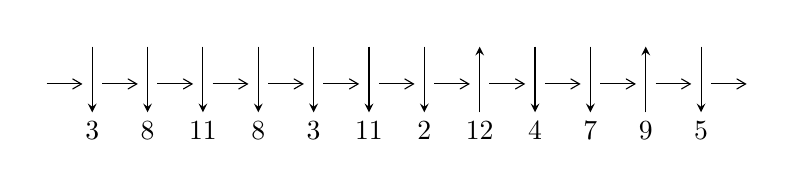
\begin{tikzpicture}[x=20pt, y=17pt]
	% nodes
	\node (C0) at (0, 0) {};
	\node (C1) at (1, 0) {};
	\node (C1U) at (1, +1) {};
	\node (C1D) at (1, -1) {3};

	\node (C2) at (2, 0) {};
	\node (C2U) at (2, +1) {};
	\node (C2D) at (2, -1) {8};

	\node (C3) at (3, 0) {};
	\node (C3U) at (3, +1) {};
	\node (C3D) at (3, -1) {11};

	\node (C4) at (4, 0) {};
	\node (C4U) at (4, +1) {};
	\node (C4D) at (4, -1) {8};

	\node (C5) at (5, 0) {};
	\node (C5U) at (5, +1) {};
	\node (C5D) at (5, -1) {3};

	\node (C6) at (6, 0) {};
	\node (C6U) at (6, +1) {};
	\node (C6D) at (6, -1) {11};

	\node (C7) at (7, 0) {};
	\node (C7U) at (7, +1) {};
	\node (C7D) at (7, -1) {2};

	\node (C8) at (8, 0) {};
	\node (C8U) at (8, +1) {};
	\node (C8D) at (8, -1) {12};

	\node (C9) at (9, 0) {};
	\node (C9U) at (9, +1) {};
	\node (C9D) at (9, -1) {4};

	\node (C10) at (10, 0) {};
	\node (C10U) at (10, +1) {};
	\node (C10D) at (10, -1) {7};

	\node (C11) at (11, 0) {};
	\node (C11U) at (11, +1) {};
	\node (C11D) at (11, -1) {9};

	\node (C12) at (12, 0) {};
	\node (C12U) at (12, +1) {};
	\node (C12D) at (12, -1) {5};
	\node (C13) at (13, 0) {};

	% arrows
	\draw[->,>={angle 60}]
	(C0) edge (C1) (C1) edge (C2) (C2) edge (C3) (C3) edge (C4) (C4) edge (C5) (C5) edge (C6) (C6) edge (C7) (C7) edge (C8) (C8) edge (C9) (C9) edge (C10) (C10) edge (C11) (C11) edge (C12) (C12) edge (C13) ;	\draw[->,>=stealth]
	(C1U) edge (C1D) (C2U) edge (C2D) (C3U) edge (C3D) (C4U) edge (C4D) (C5U) edge (C5D) (C6U) edge (C6D) (C7U) edge (C7D) (C8D) edge (C8U) (C9U) edge (C9D) (C10U) edge (C10D) (C11D) edge (C11U) (C12U) edge (C12D) ;
	\end{tikzpicture} \\
\hhline{~~} \\& 
\textbf{Solving Sequence} \\ \cline{2-2} 
 &
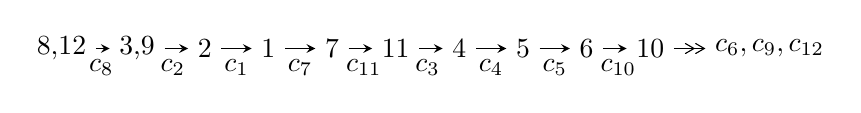
\begin{tikzpicture}[x=23pt, y=7pt]
	% node
	\node (A0) at (-1/8, 0) {8,12};
	\node (A1) at (17/16, 0) {3,9};
	\node (A2) at (17/8, 0) {2};
	\node (A3) at (25/8, 0) {1};
	\node (A4) at (33/8, 0) {7};
	\node (A5) at (41/8, 0) {11};
	\node (A6) at (49/8, 0) {4};
	\node (A7) at (57/8, 0) {5};
	\node (A8) at (65/8, 0) {6};
	\node (A9) at (73/8, 0) {10};
	\node (C1) at (1/2, -1) {$c_{8}$};
	\node (C2) at (13/8, -1) {$c_{2}$};
	\node (C3) at (21/8, -1) {$c_{1}$};
	\node (C4) at (29/8, -1) {$c_{7}$};
	\node (C5) at (37/8, -1) {$c_{11}$};
	\node (C6) at (45/8, -1) {$c_{3}$};
	\node (C7) at (53/8, -1) {$c_{4}$};
	\node (C8) at (61/8, -1) {$c_{5}$};
	\node (C9) at (69/8, -1) {$c_{10}$};
	\node (A10) at (11, 0) {$c_{6},c_{9},c_{12}$};

	% edge
	\draw[->,>=stealth]	
	(A0) edge (A1) (A1) edge (A2) (A2) edge (A3) (A3) edge (A4) (A4) edge (A5) (A5) edge (A6) (A6) edge (A7) (A7) edge (A8) (A8) edge (A9) ;
	\draw[->>,>={angle 60}]	
	(A9) edge (A10);
\end{tikzpicture} \\ 

\end{tabular} \\

\footnotetext{
The image of knot diagram is generated by the software ``\textbf{Draw programme}" developed by Andrew Bartholomew(\url{http://www.layer8.co.uk/maths/draw/index.htm\#Running-draw}), where we modified some parts for our purpose(\url{https://github.com/CATsTAILs/LinksPainter}).
}\phantom \\ \newline 
\centering \textbf{Ideals for irreducible components\footnotemark of $X_{\text{par}}$} 
 
\begin{align*}
I^u_{1}&=\langle 
u^{16}- u^{15}+6 u^{14}-5 u^{13}+13 u^{12}-10 u^{11}+8 u^{10}-9 u^9-9 u^8-4 u^7-9 u^6+8 u^4+2 u^3+9 u^2+b+u-1,\\
\phantom{I^u_{1}}&\phantom{= \langle  }u^{16}-3 u^{15}+\cdots+a+5,\;u^{18}-2 u^{17}+\cdots-8 u+1\rangle \\
I^u_{2}&=\langle 
u^{11}+2 u^{10}+6 u^9+8 u^8+12 u^7+12 u^6+9 u^5+6 u^4- u^2+b-2 u-2,\\
\phantom{I^u_{2}}&\phantom{= \langle  }- u^{11}-3 u^{10}-10 u^9-18 u^8-30 u^7-35 u^6-33 u^5-23 u^4-6 u^3+4 u^2+a+9 u+6,\\
\phantom{I^u_{2}}&\phantom{= \langle  }u^{12}+3 u^{11}+9 u^{10}+16 u^9+25 u^8+30 u^7+28 u^6+21 u^5+8 u^4- u^3-5 u^2-5 u-1\rangle \\
\\
\end{align*}
\raggedright * 2 irreducible components of $\dim_{\mathbb{C}}=0$, with total 30 representations.\\
\footnotetext{All coefficients of polynomials are rational numbers. But the coefficients are sometimes approximated in decimal forms when there is not enough margin.}
\newpage
\renewcommand{\arraystretch}{1}
\centering \section*{I. $I^u_{1}= \langle u^{16}- u^{15}+\cdots+b-1,\;u^{16}-3 u^{15}+\cdots+a+5,\;u^{18}-2 u^{17}+\cdots-8 u+1 \rangle$}
\flushleft \textbf{(i) Arc colorings}\\
\begin{tabular}{m{7pt} m{180pt} m{7pt} m{180pt} }
\flushright $a_{8}=$&$\begin{pmatrix}1\\0\end{pmatrix}$ \\
\flushright $a_{12}=$&$\begin{pmatrix}0\\u\end{pmatrix}$ \\
\flushright $a_{3}=$&$\begin{pmatrix}- u^{16}+3 u^{15}+\cdots+18 u-5\\- u^{16}+u^{15}+\cdots- u+1\end{pmatrix}$ \\
\flushright $a_{9}=$&$\begin{pmatrix}1\\- u^2\end{pmatrix}$ \\
\flushright $a_{2}=$&$\begin{pmatrix}-2 u^{16}+4 u^{15}+\cdots+17 u-4\\- u^{16}+u^{15}+\cdots- u+1\end{pmatrix}$ \\
\flushright $a_{1}=$&$\begin{pmatrix}- u^{15}+u^{14}+\cdots-10 u+1\\u^{16}- u^{15}+\cdots+3 u^3+10 u^2\end{pmatrix}$ \\
\flushright $a_{7}=$&$\begin{pmatrix}- u^{17}-5 u^{15}+\cdots+5 u+1\\- u^{16}+u^{15}+\cdots-11 u^2+u\end{pmatrix}$ \\
\flushright $a_{11}=$&$\begin{pmatrix}- u\\u^3+u\end{pmatrix}$ \\
\flushright $a_{4}=$&$\begin{pmatrix}u^{17}-2 u^{16}+\cdots+19 u-5\\- u^{17}+u^{16}+\cdots-9 u+2\end{pmatrix}$ \\
\flushright $a_{5}=$&$\begin{pmatrix}2 u^{17}-3 u^{16}+\cdots+28 u-7\\- u^{17}+u^{16}+\cdots-9 u+2\end{pmatrix}$ \\
\flushright $a_{6}=$&$\begin{pmatrix}u^{16}-2 u^{15}+\cdots-6 u-1\\u^{17}- u^{16}+\cdots+7 u-1\end{pmatrix}$ \\
\flushright $a_{10}=$&$\begin{pmatrix}- u^{17}+u^{16}+\cdots-4 u+1\\- u^{16}+u^{15}+\cdots+7 u-1\end{pmatrix}$\\&\end{tabular}
\flushleft \textbf{(ii) Obstruction class $= -1$}\\~\\
\flushleft \textbf{(iii) Cusp Shapes $= 2 u^{17}-3 u^{16}+19 u^{15}-23 u^{14}+70 u^{13}-72 u^{12}+124 u^{11}-114 u^{10}+89 u^9-89 u^8-15 u^7-26 u^6-27 u^5-2 u^4+51 u^3-15 u^2+50 u-24$}\\~\\
\newpage\renewcommand{\arraystretch}{1}
\flushleft \textbf{(iv) u-Polynomials at the component}\newline \\
\begin{tabular}{m{50pt}|m{274pt}}
Crossings & \hspace{64pt}u-Polynomials at each crossing \\
\hline $$\begin{aligned}c_{1}\end{aligned}$$&$\begin{aligned}
&u^{18}+14 u^{17}+\cdots+21504 u+4096
\end{aligned}$\\
\hline $$\begin{aligned}c_{2},c_{7}\end{aligned}$$&$\begin{aligned}
&u^{18}-16 u^{17}+\cdots+224 u-64
\end{aligned}$\\
\hline $$\begin{aligned}c_{3},c_{6},c_{10}\end{aligned}$$&$\begin{aligned}
&u^{18}+2 u^{17}+\cdots-2 u-1
\end{aligned}$\\
\hline $$\begin{aligned}c_{4},c_{12}\end{aligned}$$&$\begin{aligned}
&u^{18}+3 u^{17}+\cdots-2 u-1
\end{aligned}$\\
\hline $$\begin{aligned}c_{5}\end{aligned}$$&$\begin{aligned}
&u^{18}-5 u^{17}+\cdots-4 u+1
\end{aligned}$\\
\hline $$\begin{aligned}c_{8},c_{11}\end{aligned}$$&$\begin{aligned}
&u^{18}+2 u^{17}+\cdots+8 u+1
\end{aligned}$\\
\hline $$\begin{aligned}c_{9}\end{aligned}$$&$\begin{aligned}
&u^{18}- u^{17}+\cdots-120 u-61
\end{aligned}$\\
\hline
\end{tabular}\\~\\
\newpage\renewcommand{\arraystretch}{1}
\flushleft \textbf{(v) Riley Polynomials at the component}\newline \\
\begin{tabular}{m{50pt}|m{274pt}}
Crossings & \hspace{64pt}Riley Polynomials at each crossing \\
\hline $$\begin{aligned}c_{1}\end{aligned}$$&$\begin{aligned}
&y^{18}+82 y^{17}+\cdots-437256192 y+16777216
\end{aligned}$\\
\hline $$\begin{aligned}c_{2},c_{7}\end{aligned}$$&$\begin{aligned}
&y^{18}-14 y^{17}+\cdots-21504 y+4096
\end{aligned}$\\
\hline $$\begin{aligned}c_{3},c_{6},c_{10}\end{aligned}$$&$\begin{aligned}
&y^{18}+28 y^{17}+\cdots-18 y+1
\end{aligned}$\\
\hline $$\begin{aligned}c_{4},c_{12}\end{aligned}$$&$\begin{aligned}
&y^{18}+35 y^{17}+\cdots+20 y+1
\end{aligned}$\\
\hline $$\begin{aligned}c_{5}\end{aligned}$$&$\begin{aligned}
&y^{18}-45 y^{17}+\cdots-20 y+1
\end{aligned}$\\
\hline $$\begin{aligned}c_{8},c_{11}\end{aligned}$$&$\begin{aligned}
&y^{18}+14 y^{17}+\cdots-32 y+1
\end{aligned}$\\
\hline $$\begin{aligned}c_{9}\end{aligned}$$&$\begin{aligned}
&y^{18}+33 y^{17}+\cdots+24762 y+3721
\end{aligned}$\\
\hline
\end{tabular}\\~\\
\newpage\flushleft \textbf{(vi) Complex Volumes and Cusp Shapes}
$$\begin{array}{c|c|c}  
\text{Solutions to }I^u_{1}& \I (\text{vol} + \sqrt{-1}CS) & \text{Cusp shape}\\
 \hline 
\begin{aligned}
u &= \phantom{-}0.957035 + 0.038927 I \\
a &= \phantom{-}1.29444 - 2.14220 I \\
b &= -1.52646 + 1.38753 I\end{aligned}
 & \phantom{-}12.15720 + 5.50571 I & -6.58833 - 2.14870 I \\ \hline\begin{aligned}
u &= \phantom{-}0.957035 - 0.038927 I \\
a &= \phantom{-}1.29444 + 2.14220 I \\
b &= -1.52646 - 1.38753 I\end{aligned}
 & \phantom{-}12.15720 - 5.50571 I & -6.58833 + 2.14870 I \\ \hline\begin{aligned}
u &= -0.292699 + 1.060130 I \\
a &= \phantom{-}0.130715 - 0.442861 I \\
b &= -0.090901 + 0.653348 I\end{aligned}
 & -0.84836 - 1.94165 I & -6.35139 + 2.74428 I \\ \hline\begin{aligned}
u &= -0.292699 - 1.060130 I \\
a &= \phantom{-}0.130715 + 0.442861 I \\
b &= -0.090901 - 0.653348 I\end{aligned}
 & -0.84836 + 1.94165 I & -6.35139 - 2.74428 I \\ \hline\begin{aligned}
u &= \phantom{-}0.074993 + 1.132910 I \\
a &= \phantom{-}0.751791 + 0.803103 I \\
b &= \phantom{-}0.794717 - 0.290190 I\end{aligned}
 & -3.55462 + 1.02828 I & -12.61847 - 1.28084 I \\ \hline\begin{aligned}
u &= \phantom{-}0.074993 - 1.132910 I \\
a &= \phantom{-}0.751791 - 0.803103 I \\
b &= \phantom{-}0.794717 + 0.290190 I\end{aligned}
 & -3.55462 - 1.02828 I & -12.61847 + 1.28084 I \\ \hline\begin{aligned}
u &= -0.796441 + 0.291195 I \\
a &= \phantom{-}0.151574 + 0.889968 I \\
b &= -0.775836 - 0.472537 I\end{aligned}
 & \phantom{-}1.24471 - 1.98200 I & -5.60868 + 9.18970 I \\ \hline\begin{aligned}
u &= -0.796441 - 0.291195 I \\
a &= \phantom{-}0.151574 - 0.889968 I \\
b &= -0.775836 + 0.472537 I\end{aligned}
 & \phantom{-}1.24471 + 1.98200 I & -5.60868 - 9.18970 I \\ \hline\begin{aligned}
u &= \phantom{-}0.147448 + 1.249270 I \\
a &= -1.46732 - 1.39599 I \\
b &= -1.62783 + 0.04234 I\end{aligned}
 & -11.88260 + 2.10947 I & -15.7034 - 5.8224 I \\ \hline\begin{aligned}
u &= \phantom{-}0.147448 - 1.249270 I \\
a &= -1.46732 + 1.39599 I \\
b &= -1.62783 - 0.04234 I\end{aligned}
 & -11.88260 - 2.10947 I & -15.7034 + 5.8224 I\\
 \hline 
 \end{array}$$\newpage$$\begin{array}{c|c|c}  
\text{Solutions to }I^u_{1}& \I (\text{vol} + \sqrt{-1}CS) & \text{Cusp shape}\\
 \hline 
\begin{aligned}
u &= \phantom{-}0.490413 + 1.272180 I \\
a &= \phantom{-}1.140910 + 0.046544 I \\
b &= -1.42593 - 1.40587 I\end{aligned}
 & \phantom{-}8.34549 - 0.36039 I & -9.48611 - 0.73252 I \\ \hline\begin{aligned}
u &= \phantom{-}0.490413 - 1.272180 I \\
a &= \phantom{-}1.140910 - 0.046544 I \\
b &= -1.42593 + 1.40587 I\end{aligned}
 & \phantom{-}8.34549 + 0.36039 I & -9.48611 + 0.73252 I \\ \hline\begin{aligned}
u &= \phantom{-}0.458123 + 1.327850 I \\
a &= -0.80670 - 2.00900 I \\
b &= -1.59701 + 1.33472 I\end{aligned}
 & \phantom{-}7.89248 + 10.55150 I & -10.01468 - 4.70572 I \\ \hline\begin{aligned}
u &= \phantom{-}0.458123 - 1.327850 I \\
a &= -0.80670 + 2.00900 I \\
b &= -1.59701 - 1.33472 I\end{aligned}
 & \phantom{-}7.89248 - 10.55150 I & -10.01468 + 4.70572 I \\ \hline\begin{aligned}
u &= -0.35310 + 1.38486 I \\
a &= -0.684948 + 0.964946 I \\
b &= -1.194280 - 0.456860 I\end{aligned}
 & -4.04162 - 6.18627 I & -15.0481 + 5.4779 I \\ \hline\begin{aligned}
u &= -0.35310 - 1.38486 I \\
a &= -0.684948 - 0.964946 I \\
b &= -1.194280 + 0.456860 I\end{aligned}
 & -4.04162 + 6.18627 I & -15.0481 - 5.4779 I \\ \hline\begin{aligned}
u &= \phantom{-}0.443581\phantom{ +0.000000I} \\
a &= \phantom{-}1.93499\phantom{ +0.000000I} \\
b &= -1.59894\phantom{ +0.000000I}\end{aligned}
 & -8.07946\phantom{ +0.000000I} & -1.20520\phantom{ +0.000000I} \\ \hline\begin{aligned}
u &= \phantom{-}0.184865\phantom{ +0.000000I} \\
a &= -1.95591\phantom{ +0.000000I} \\
b &= \phantom{-}0.485984\phantom{ +0.000000I}\end{aligned}
 & -0.676311\phantom{ +0.000000I} & -14.9570\phantom{ +0.000000I}\\
 \hline 
 \end{array}$$\newpage\newpage\renewcommand{\arraystretch}{1}
\centering \section*{II. $I^u_{2}= \langle u^{11}+2 u^{10}+\cdots+b-2,\;- u^{11}-3 u^{10}+\cdots+a+6,\;u^{12}+3 u^{11}+\cdots-5 u-1 \rangle$}
\flushleft \textbf{(i) Arc colorings}\\
\begin{tabular}{m{7pt} m{180pt} m{7pt} m{180pt} }
\flushright $a_{8}=$&$\begin{pmatrix}1\\0\end{pmatrix}$ \\
\flushright $a_{12}=$&$\begin{pmatrix}0\\u\end{pmatrix}$ \\
\flushright $a_{3}=$&$\begin{pmatrix}u^{11}+3 u^{10}+\cdots-9 u-6\\- u^{11}-2 u^{10}-6 u^9-8 u^8-12 u^7-12 u^6-9 u^5-6 u^4+u^2+2 u+2\end{pmatrix}$ \\
\flushright $a_{9}=$&$\begin{pmatrix}1\\- u^2\end{pmatrix}$ \\
\flushright $a_{2}=$&$\begin{pmatrix}u^{10}+4 u^9+10 u^8+18 u^7+23 u^6+24 u^5+17 u^4+6 u^3-3 u^2-7 u-4\\- u^{11}-2 u^{10}-6 u^9-8 u^8-12 u^7-12 u^6-9 u^5-6 u^4+u^2+2 u+2\end{pmatrix}$ \\
\flushright $a_{1}=$&$\begin{pmatrix}-2 u^{11}-6 u^{10}+\cdots+14 u+10\\- u^{10}-2 u^9-5 u^8-5 u^7-5 u^6-2 u^5+2 u^4+3 u^3+4 u^2+u-2\end{pmatrix}$ \\
\flushright $a_{7}=$&$\begin{pmatrix}- u^{11}-5 u^{10}+\cdots+15 u+8\\- u^{10}-2 u^9-5 u^8-6 u^7-6 u^6-5 u^5+u^3+3 u^2+2 u-2\end{pmatrix}$ \\
\flushright $a_{11}=$&$\begin{pmatrix}- u\\u^3+u\end{pmatrix}$ \\
\flushright $a_{4}=$&$\begin{pmatrix}u^{11}+4 u^{10}+\cdots-10 u-6\\u^{10}+2 u^9+5 u^8+6 u^7+6 u^6+5 u^5- u^3-3 u^2-2 u+1\end{pmatrix}$ \\
\flushright $a_{5}=$&$\begin{pmatrix}u^{11}+3 u^{10}+\cdots-8 u-7\\u^{10}+2 u^9+5 u^8+6 u^7+6 u^6+5 u^5- u^3-3 u^2-2 u+1\end{pmatrix}$ \\
\flushright $a_{6}=$&$\begin{pmatrix}- u^{11}-4 u^{10}+\cdots+14 u+8\\u^{11}+2 u^{10}+6 u^9+8 u^8+12 u^7+12 u^6+9 u^5+6 u^4- u^2-2 u-3\end{pmatrix}$ \\
\flushright $a_{10}=$&$\begin{pmatrix}3 u^{11}+8 u^{10}+\cdots-5 u-4\\- u^{10}-4 u^9+\cdots+7 u+3\end{pmatrix}$\\&\end{tabular}
\flushleft \textbf{(ii) Obstruction class $= 1$}\\~\\
\flushleft \textbf{(iii) Cusp Shapes $= 7 u^{11}+15 u^{10}+48 u^9+70 u^8+112 u^7+121 u^6+105 u^5+81 u^4+18 u^3-2 u^2-21 u-29$}\\~\\
\newpage\renewcommand{\arraystretch}{1}
\flushleft \textbf{(iv) u-Polynomials at the component}\newline \\
\begin{tabular}{m{50pt}|m{274pt}}
Crossings & \hspace{64pt}u-Polynomials at each crossing \\
\hline $$\begin{aligned}c_{1}\end{aligned}$$&$\begin{aligned}
&u^{12}-14 u^{11}+\cdots-67 u+9
\end{aligned}$\\
\hline $$\begin{aligned}c_{2}\end{aligned}$$&$\begin{aligned}
&u^{12}+2 u^{11}+\cdots- u+3
\end{aligned}$\\
\hline $$\begin{aligned}c_{3},c_{10}\end{aligned}$$&$\begin{aligned}
&u^{12}- u^{11}-2 u^{10}- u^9+2 u^8+4 u^7-2 u^6+3 u^5-3 u^4+4 u^3-2 u^2+u-1
\end{aligned}$\\
\hline $$\begin{aligned}c_{4},c_{12}\end{aligned}$$&$\begin{aligned}
&u^{12}+2 u^{11}- u^{10}- u^9+6 u^8-3 u^7+u^6+5 u^5-5 u^4+7 u^3-5 u^2+3 u-1
\end{aligned}$\\
\hline $$\begin{aligned}c_{5}\end{aligned}$$&$\begin{aligned}
&u^{12}+14 u^{11}+\cdots+3 u+1
\end{aligned}$\\
\hline $$\begin{aligned}c_{6}\end{aligned}$$&$\begin{aligned}
&u^{12}+u^{11}-2 u^{10}+u^9+2 u^8-4 u^7-2 u^6-3 u^5-3 u^4-4 u^3-2 u^2- u-1
\end{aligned}$\\
\hline $$\begin{aligned}c_{7}\end{aligned}$$&$\begin{aligned}
&u^{12}-2 u^{11}+\cdots+u+3
\end{aligned}$\\
\hline $$\begin{aligned}c_{8}\end{aligned}$$&$\begin{aligned}
&u^{12}+3 u^{11}+\cdots-5 u-1
\end{aligned}$\\
\hline $$\begin{aligned}c_{9}\end{aligned}$$&$\begin{aligned}
&u^{12}-2 u^{10}-6 u^9+13 u^8+u^7+2 u^6-9 u^5-8 u^4+9 u^3-4 u^2+5 u-3
\end{aligned}$\\
\hline $$\begin{aligned}c_{11}\end{aligned}$$&$\begin{aligned}
&u^{12}-3 u^{11}+\cdots+5 u-1
\end{aligned}$\\
\hline
\end{tabular}\\~\\
\newpage\renewcommand{\arraystretch}{1}
\flushleft \textbf{(v) Riley Polynomials at the component}\newline \\
\begin{tabular}{m{50pt}|m{274pt}}
Crossings & \hspace{64pt}Riley Polynomials at each crossing \\
\hline $$\begin{aligned}c_{1}\end{aligned}$$&$\begin{aligned}
&y^{12}-22 y^{11}+\cdots+29 y+81
\end{aligned}$\\
\hline $$\begin{aligned}c_{2},c_{7}\end{aligned}$$&$\begin{aligned}
&y^{12}-14 y^{11}+\cdots-67 y+9
\end{aligned}$\\
\hline $$\begin{aligned}c_{3},c_{6},c_{10}\end{aligned}$$&$\begin{aligned}
&y^{12}-5 y^{11}+\cdots+3 y+1
\end{aligned}$\\
\hline $$\begin{aligned}c_{4},c_{12}\end{aligned}$$&$\begin{aligned}
&y^{12}-6 y^{11}+\cdots+y+1
\end{aligned}$\\
\hline $$\begin{aligned}c_{5}\end{aligned}$$&$\begin{aligned}
&y^{12}-30 y^{11}+\cdots+21 y+1
\end{aligned}$\\
\hline $$\begin{aligned}c_{8},c_{11}\end{aligned}$$&$\begin{aligned}
&y^{12}+9 y^{11}+\cdots-15 y+1
\end{aligned}$\\
\hline $$\begin{aligned}c_{9}\end{aligned}$$&$\begin{aligned}
&y^{12}-4 y^{11}+\cdots- y+9
\end{aligned}$\\
\hline
\end{tabular}\\~\\
\newpage\flushleft \textbf{(vi) Complex Volumes and Cusp Shapes}
$$\begin{array}{c|c|c}  
\text{Solutions to }I^u_{2}& \I (\text{vol} + \sqrt{-1}CS) & \text{Cusp shape}\\
 \hline 
\begin{aligned}
u &= -0.945559 + 0.176012 I \\
a &= \phantom{-}0.384985 + 0.661564 I \\
b &= -0.934205 - 0.378092 I\end{aligned}
 & \phantom{-}1.63828 - 1.45323 I & \phantom{-}1.054104 + 0.917158 I \\ \hline\begin{aligned}
u &= -0.945559 - 0.176012 I \\
a &= \phantom{-}0.384985 - 0.661564 I \\
b &= -0.934205 + 0.378092 I\end{aligned}
 & \phantom{-}1.63828 + 1.45323 I & \phantom{-}1.054104 - 0.917158 I \\ \hline\begin{aligned}
u &= -0.083486 + 1.161420 I \\
a &= \phantom{-}1.36019 - 1.88104 I \\
b &= \phantom{-}1.71485 + 0.22346 I\end{aligned}
 & -11.61070 - 1.25522 I & -12.48094 - 2.13033 I \\ \hline\begin{aligned}
u &= -0.083486 - 1.161420 I \\
a &= \phantom{-}1.36019 + 1.88104 I \\
b &= \phantom{-}1.71485 - 0.22346 I\end{aligned}
 & -11.61070 + 1.25522 I & -12.48094 + 2.13033 I \\ \hline\begin{aligned}
u &= \phantom{-}0.262959 + 1.174910 I \\
a &= -0.73282 + 1.30130 I \\
b &= \phantom{-}0.886932 - 0.447310 I\end{aligned}
 & -8.28259 + 3.18829 I & -11.15779 - 3.99090 I \\ \hline\begin{aligned}
u &= \phantom{-}0.262959 - 1.174910 I \\
a &= -0.73282 - 1.30130 I \\
b &= \phantom{-}0.886932 + 0.447310 I\end{aligned}
 & -8.28259 - 3.18829 I & -11.15779 + 3.99090 I \\ \hline\begin{aligned}
u &= -0.451022 + 1.172390 I \\
a &= -0.0134217 + 0.1288200 I \\
b &= -0.609088 + 0.508190 I\end{aligned}
 & -1.38760 - 3.47878 I & -6.82613 + 4.40874 I \\ \hline\begin{aligned}
u &= -0.451022 - 1.172390 I \\
a &= -0.0134217 - 0.1288200 I \\
b &= -0.609088 - 0.508190 I\end{aligned}
 & -1.38760 + 3.47878 I & -6.82613 - 4.40874 I \\ \hline\begin{aligned}
u &= \phantom{-}0.612728\phantom{ +0.000000I} \\
a &= -2.21290\phantom{ +0.000000I} \\
b &= \phantom{-}0.702300\phantom{ +0.000000I}\end{aligned}
 & -4.82802\phantom{ +0.000000I} & -5.83830\phantom{ +0.000000I} \\ \hline\begin{aligned}
u &= -0.45888 + 1.40396 I \\
a &= -0.414406 + 0.891813 I \\
b &= -1.172970 - 0.328171 I\end{aligned}
 & -3.32828 - 6.54831 I & -6.31944 + 10.84380 I\\
 \hline 
 \end{array}$$\newpage$$\begin{array}{c|c|c}  
\text{Solutions to }I^u_{2}& \I (\text{vol} + \sqrt{-1}CS) & \text{Cusp shape}\\
 \hline 
\begin{aligned}
u &= -0.45888 - 1.40396 I \\
a &= -0.414406 - 0.891813 I \\
b &= -1.172970 + 0.328171 I\end{aligned}
 & -3.32828 + 6.54831 I & -6.31944 - 10.84380 I \\ \hline\begin{aligned}
u &= -0.260752\phantom{ +0.000000I} \\
a &= -3.95615\phantom{ +0.000000I} \\
b &= \phantom{-}1.52667\phantom{ +0.000000I}\end{aligned}
 & -8.44787\phantom{ +0.000000I} & -23.7010\phantom{ +0.000000I}\\
 \hline 
 \end{array}$$\newpage
\newpage\renewcommand{\arraystretch}{1}
\centering \section*{ III. u-Polynomials}
\begin{tabular}{m{50pt}|m{274pt}}
Crossings & \hspace{64pt}u-Polynomials at each crossing \\
\hline $$\begin{aligned}c_{1}\end{aligned}$$&$\begin{aligned}
&(u^{12}-14 u^{11}+\cdots-67 u+9)(u^{18}+14 u^{17}+\cdots+21504 u+4096)
\end{aligned}$\\
\hline $$\begin{aligned}c_{2}\end{aligned}$$&$\begin{aligned}
&(u^{12}+2 u^{11}+\cdots- u+3)(u^{18}-16 u^{17}+\cdots+224 u-64)
\end{aligned}$\\
\hline $$\begin{aligned}c_{3},c_{10}\end{aligned}$$&$\begin{aligned}
&(u^{12}- u^{11}-2 u^{10}- u^9+2 u^8+4 u^7-2 u^6+3 u^5-3 u^4+4 u^3-2 u^2+u-1)\\
&\cdot(u^{18}+2 u^{17}+\cdots-2 u-1)
\end{aligned}$\\
\hline $$\begin{aligned}c_{4},c_{12}\end{aligned}$$&$\begin{aligned}
&(u^{12}+2 u^{11}- u^{10}- u^9+6 u^8-3 u^7+u^6+5 u^5-5 u^4+7 u^3-5 u^2+3 u-1)\\
&\cdot(u^{18}+3 u^{17}+\cdots-2 u-1)
\end{aligned}$\\
\hline $$\begin{aligned}c_{5}\end{aligned}$$&$\begin{aligned}
&(u^{12}+14 u^{11}+\cdots+3 u+1)(u^{18}-5 u^{17}+\cdots-4 u+1)
\end{aligned}$\\
\hline $$\begin{aligned}c_{6}\end{aligned}$$&$\begin{aligned}
&(u^{12}+u^{11}-2 u^{10}+u^9+2 u^8-4 u^7-2 u^6-3 u^5-3 u^4-4 u^3-2 u^2- u-1)\\
&\cdot(u^{18}+2 u^{17}+\cdots-2 u-1)
\end{aligned}$\\
\hline $$\begin{aligned}c_{7}\end{aligned}$$&$\begin{aligned}
&(u^{12}-2 u^{11}+\cdots+u+3)(u^{18}-16 u^{17}+\cdots+224 u-64)
\end{aligned}$\\
\hline $$\begin{aligned}c_{8}\end{aligned}$$&$\begin{aligned}
&(u^{12}+3 u^{11}+\cdots-5 u-1)(u^{18}+2 u^{17}+\cdots+8 u+1)
\end{aligned}$\\
\hline $$\begin{aligned}c_{9}\end{aligned}$$&$\begin{aligned}
&(u^{12}-2 u^{10}-6 u^9+13 u^8+u^7+2 u^6-9 u^5-8 u^4+9 u^3-4 u^2+5 u-3)\\
&\cdot(u^{18}- u^{17}+\cdots-120 u-61)
\end{aligned}$\\
\hline $$\begin{aligned}c_{11}\end{aligned}$$&$\begin{aligned}
&(u^{12}-3 u^{11}+\cdots+5 u-1)(u^{18}+2 u^{17}+\cdots+8 u+1)
\end{aligned}$\\
\hline
\end{tabular}\newpage\renewcommand{\arraystretch}{1}
\centering \section*{ IV. Riley Polynomials}
\begin{tabular}{m{50pt}|m{274pt}}
Crossings & \hspace{64pt}Riley Polynomials at each crossing \\
\hline $$\begin{aligned}c_{1}\end{aligned}$$&$\begin{aligned}
&(y^{12}-22 y^{11}+\cdots+29 y+81)\\
&\cdot(y^{18}+82 y^{17}+\cdots-437256192 y+16777216)
\end{aligned}$\\
\hline $$\begin{aligned}c_{2},c_{7}\end{aligned}$$&$\begin{aligned}
&(y^{12}-14 y^{11}+\cdots-67 y+9)(y^{18}-14 y^{17}+\cdots-21504 y+4096)
\end{aligned}$\\
\hline $$\begin{aligned}c_{3},c_{6},c_{10}\end{aligned}$$&$\begin{aligned}
&(y^{12}-5 y^{11}+\cdots+3 y+1)(y^{18}+28 y^{17}+\cdots-18 y+1)
\end{aligned}$\\
\hline $$\begin{aligned}c_{4},c_{12}\end{aligned}$$&$\begin{aligned}
&(y^{12}-6 y^{11}+\cdots+y+1)(y^{18}+35 y^{17}+\cdots+20 y+1)
\end{aligned}$\\
\hline $$\begin{aligned}c_{5}\end{aligned}$$&$\begin{aligned}
&(y^{12}-30 y^{11}+\cdots+21 y+1)(y^{18}-45 y^{17}+\cdots-20 y+1)
\end{aligned}$\\
\hline $$\begin{aligned}c_{8},c_{11}\end{aligned}$$&$\begin{aligned}
&(y^{12}+9 y^{11}+\cdots-15 y+1)(y^{18}+14 y^{17}+\cdots-32 y+1)
\end{aligned}$\\
\hline $$\begin{aligned}c_{9}\end{aligned}$$&$\begin{aligned}
&(y^{12}-4 y^{11}+\cdots- y+9)(y^{18}+33 y^{17}+\cdots+24762 y+3721)
\end{aligned}$\\
\hline
\end{tabular}
\vskip 2pc
\end{document}